\clearpage\section{Architecture}

My project is not just a language and a compiler for it, but rather a much larger ecosystem. It needs to store, compile, and run scripts. To achieve this, I designed a multi-component architecture depicted in figure \ref{fig:comp_arch}.

\begin{figure}[h]
    \centering
    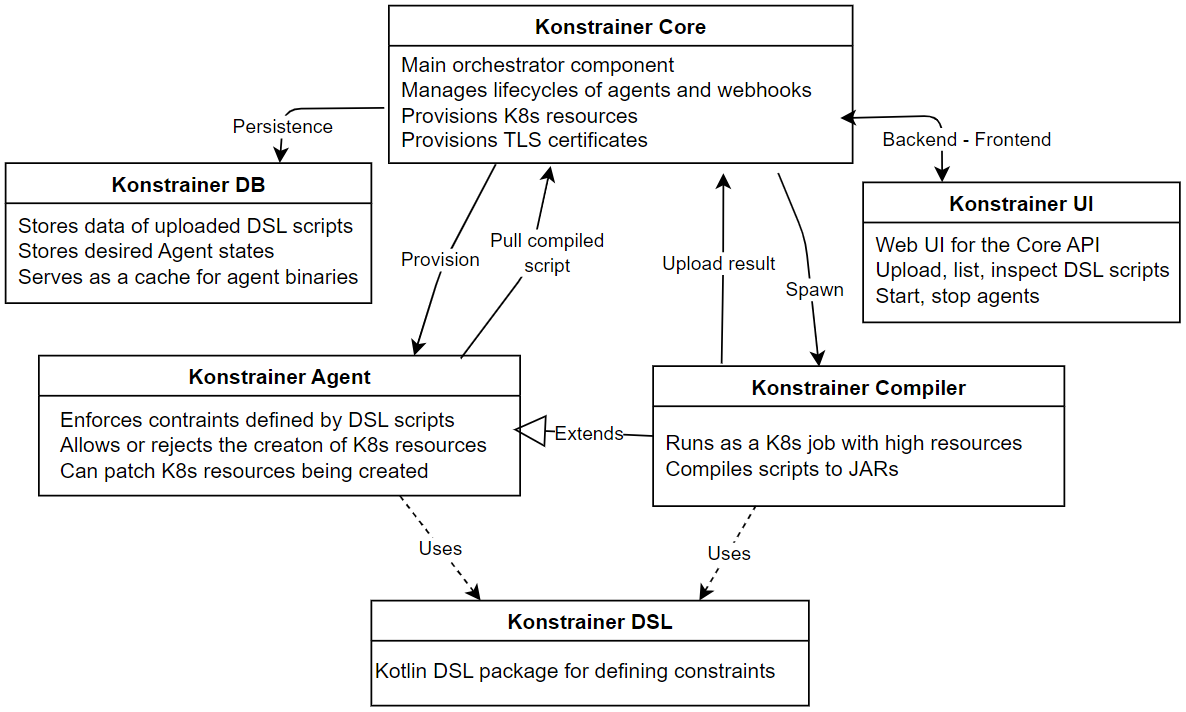
\includegraphics[width=130mm, keepaspectratio]{content/75_implementation/xarch.png}
    \caption{Complex architecture plan}
    \label{fig:comp_arch}
\end{figure}

The main component in this setup is the Konstrainer Core. This is an HTTP API server managing the whole platform. DSL scripts can be uploaded to it, and serves as a store for the uploaded and compiled DSL instances. It handles all tasks related to compiling, spawning, configuring, and destroying agents. Most importantly it manages the TLS certificates and Kubernetes resources for the agents, which are crucial parts of the agent lifecycle.

In Kubernetes, webhooks need to communicate with the Kubernetes API on a secured connection. To achieve this, Konstrainer Agent instances require a TLS certificate, and need to serve request using the HTTPS protocol. This certificate can be self-signed, but in the webhook creation request the root CA of the certificate must be sent to the Kubernetes API. After this, the Kubernetes API will trust the certificate of the webhook.

\subsection{Compiler}

Since my DSL is a Kotlin library


TODO mention agent deletion
When an Agent is deleted there is a cleanup job to do. All the created Kubernetes resources associated with the given Agent must be deleted alongside with the \emph{WebhookConfiguration}. The deletion of the \emph{deployment}, \emph{service} and \emph{WebhookConfiguration} must be atomic.


The status of the DSL instance represents the compilation state of the instance, whether it is being compiled, successfully compiled, or outdated and needs to be recompiled.

Caching the compiled DSL instances is very important. A DSL instances are compiled to JVM byte code using gradle, so compilation can take long. Compiling a DSL before each launch of an agent would significantly increase the startup time of the agent. A long startup time would mean a relatively long outage when the pod of an already existing agent gets destroyed. This could happen for many reasons, such as the pod gets evicted, deleted manually by an administrator or just simply encounters a fatal error.

An agent is a webserver that runs a DSL instance and implements a webhook. The core component spawns an agent for each deployed DSL instance.

The agent is implemented as a lightweight Ktor server. It loads a compiled Dsl class at startup time. The configuration of the agent is done by the core component.

The compilation task must be decoupled from the other components, because it is a short, but resource intensive task. Keeping it together with either the core or the agent would not be wise, since they are relatively lightweight components. Increasing the resources allocated for these components would waste expensive resources on the node. Keeping them low would result in very slow compilation times, or OOMKilled errors for the components compiling the DSL. An OOMKilled status means that the Pod tried to use more memory than its limit.
